\documentclass{beamer}
%\usepackage[size=a4]{beamerposter}

\usepackage{default}
\usepackage{epsf}
\usetheme{Malmoe}
\usecolortheme{seagull}
\usepackage{multicol}
\usepackage{subfig}
\usepackage{siunitx}
\usepackage{tikz}
\usepackage{lipsum}
%\usepackage{wrapfig}

\newcommand\Fontva{\fontsize{22}{7.2}\selectfont}
\newcommand\Fontvb{\fontsize{16}{7.2}\selectfont}

\usetikzlibrary{fit,shapes,arrows,calc,positioning}

%\newcommand*{\fnrule}{\rule{0.15\paperwidth}{0.4pt}}
%\newcommand*{\fnrule}{\rule{\paperwidth}{0.4pt}}


\begin{document}

\title[The Los Alamos Proton Storage Ring] % (optional, only for long titles)
{The Los Alamos Proton Storage Ring}
%\subtitle{Multithreaded pyzgoubi and AC-Dipole update}
\author[Abell \& Hock] % (optional, for multiple authors)
{Dan Abell and Kiel Hock} %, Fran\c{c}ois~M\'eot\inst{1}}
%\institute[MCR Group Meeting] % (optional)
%{
%  \inst{1}%
%  Collider-Accelerator Department\\
%  Brookhaven National Laboratory
%  }
\date[KPT 2004]{08/26/2019} % (optional)
%{MCR Group Meeting}
\frame{\titlepage}


\begin{frame}
\frametitle{Table of Contents}
\tableofcontents
\end{frame}

%:The Los Alamos PSR
\section{The Los Alamos PSR}

\begin{frame}
\hspace{-4em}
\begin{minipage}{0.7\textwidth}
\begin{figure}
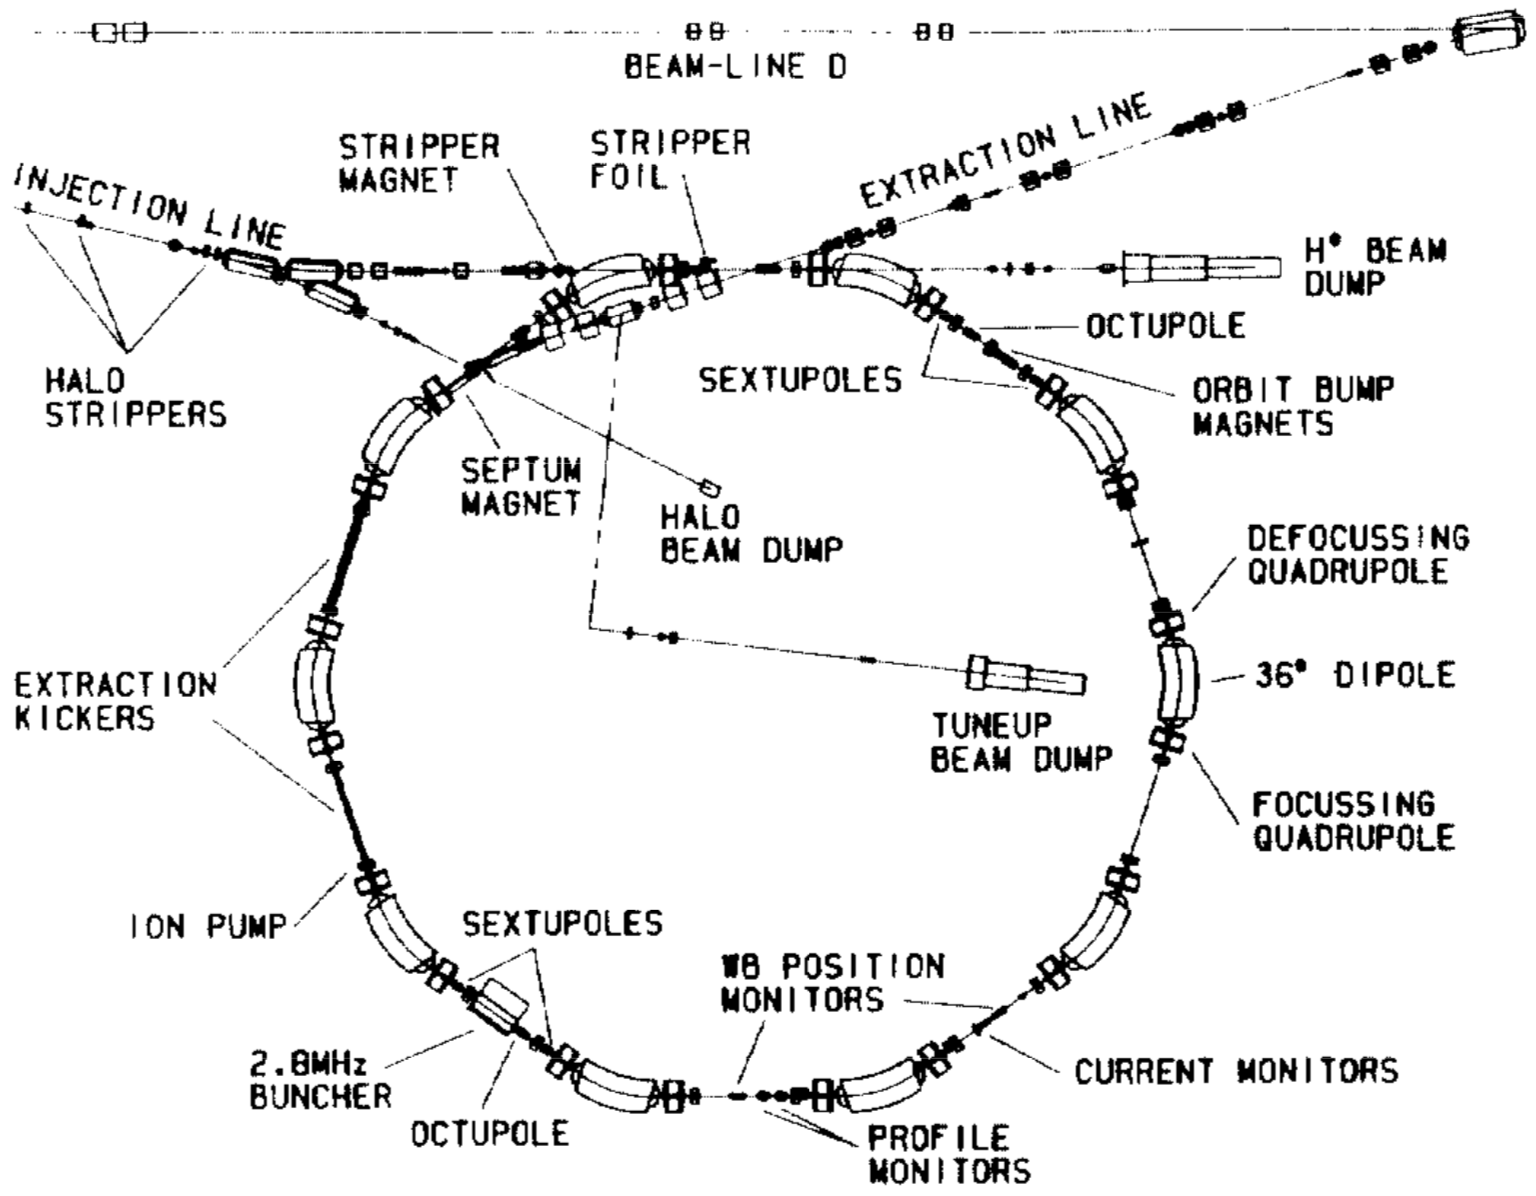
\includegraphics[trim={0 0 0 40}, clip, scale=0.22]{PAC1987_0825}
\caption{Layout of the 10-cell PSR.}
\end{figure}
\end{minipage}
\begin{minipage}{0.42\textwidth}
The LA PSR is a \SI{797}{MeV} proton storage ring with
\begin{itemize}
\item 10 dipoles,
\item 20 quadrupoles,
\item two pairs of sextupoles for chromaticity correction.
\end{itemize}
\end{minipage}
\footnoterule
\tiny
\cite{GPL} Lawrence, G. (1987).
           Performance of the Los Alamos Proton Storage Ring. PAC'1987.
\end{frame}


\section{0:\,Integration Step}
\begin{frame}
The integration step is a very important parameter for ray tracing.
\begin{itemize}
\item Go into Ex-0-FirstSteps and open the zgoubi input file, zgoubi.dat.
\item OBJET5 is used for tune calculations.
\item 'SCALING' keyword sets sextupoles fields to zero.
\item The lattice proceeds SCALING until you reach the FIT2 keyword.
\begin{itemize}
\item FIT2 is finding the closed orbit.
\end{itemize}
\item Rebelote is configured to change the integration step size in the quadrupoles (remember the sextupoles were turned off with scaling).
\end{itemize}
\tiny
\hspace*{0.2\textwidth}
\begin{minipage}{0.2\textwidth}


'REBELOTE'
                                                                   
3 1.1 0 1

1

MULTIPOL 60  5 2 1
\end{minipage}
\hspace{0.1\textwidth}
\begin{minipage}{0.4\textwidth}
 'MULTIPOL'  QUAD  QF    

0  .Quad

50.000  10.000  0.  1.95  0.  0.  0.  0.  0.  0.  0.  0.

0.000   0.00   0.  1.00  0.  0.  0.  0.  0.  0.  0.

6  0.1122 6.2671 -1.4982 3.5882 -2.1209 1.723

0.000   0.00   0.  1.00  0.  0.  0.  0.  0.  0.  0.

6  0.1122 6.2671 -1.4982 3.5882 -2.1209 1.723

0.  0.  0.  0.  0.  0.  0.  0.  0.  0.

2.0  ! cm

1 0. 0. 0.
\end{minipage}
\end{frame}

\begin{frame}
\hspace*{-2em}
\begin{minipage}{0.5\textwidth}
\begin{itemize}
\small
\item You should have found that XPAS$<<$QL (50~cm) is ideal.
\item If you use too small a step size, you pay the price of slower run times without improved accuracy.
\item Ideal step size XPAS$\sim$1
\item Plot on top right shows a comparison of resulting tunes with corresponding step size.
\item Plot on lower right shows a comparison of resulting run time with corresponding quadrupole step size.
\end{itemize}
\end{minipage}
\begin{minipage}{0.5\textwidth}
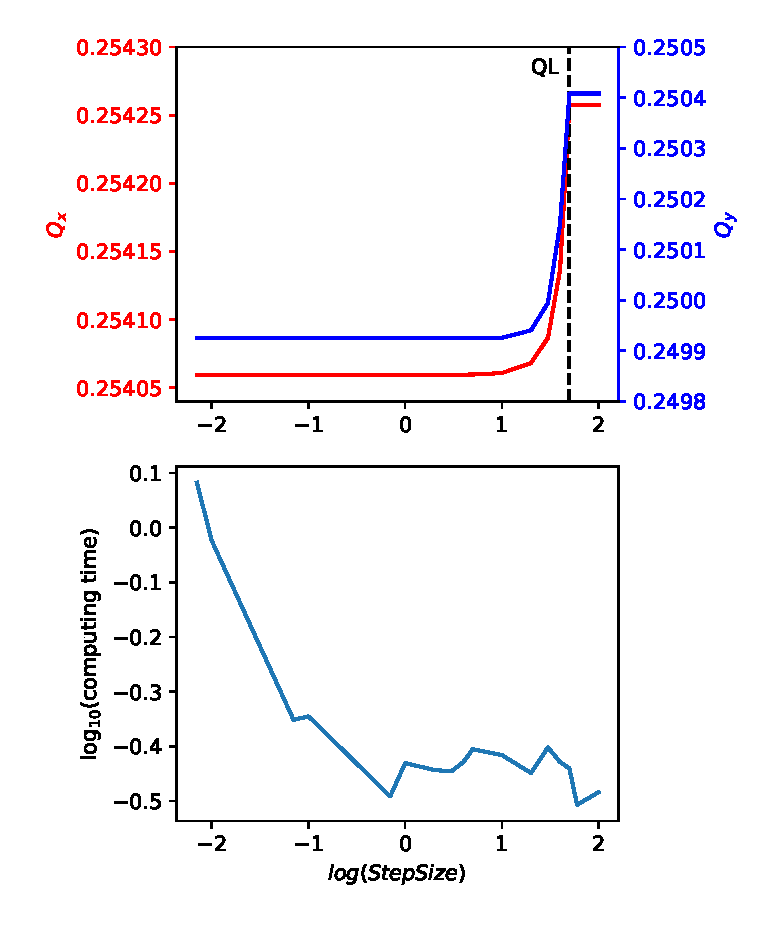
\includegraphics[width=1.0\linewidth]{Int_step.eps}
\end{minipage}
\end{frame}

\section{1:\,Chromaticity scan}
\begin{frame}
\frametitle{1-Chromaticity scan}
This file executes a chromaticity scan to match experimental data.\\
Open the zgoubi.dat file in the folder Ex-2-Chrom.\\
At line 102 there is a routine for finding the closed orbit:
\tiny

 'FIT2'
2  save

1 30 0 [-1.,+1.]

1 31 0 [-100.,+100.]

2  1.D-11  9999

3.1  1  2  \#End 0. 1. 0   ! Yf = Yi

3.1  1  3  \#End 0. 1. 0   ! Tf = Ti

\normalsize
After this routine executes, the MATRIX command is called which calculates the tunes.
\end{frame}
\begin{frame}
The chromaticity scan is done using REBELOTE (it means do it again). \\
The settings it inputs mean that it will go through the lattice 4 times and change OBJET 35 (1+$\delta_p$) to the values listed after\\
\tiny
 'REBELOTE'

4 1.1 0 1

1

OBJET 35  1.001  0.999  1.0001  0.9999

\normalsize
How do the tunes compare to the experimental data?\\
\begin{center}
\begin{tabular}{ccc}
$\delta$  &$\nu_x$  &$\nu_y$\\
\hline
0		  &2.2540596&2.2499258\\
$10^{-3}$ &2.2529848&2.2486430\\
$-10^{-3}$&2.2551372&2.2512124\\
$10^{-4}$ &2.2539520&2.2497974\\
$-10^{-4}$&2.2541673&2.2500543\\
\end{tabular}
\end{center}
\end{frame}



\section{2:\,Exploring the Optics}

\begin{frame}
\frametitle{2:\,Exploring the Optics}
In the folder labeled Ex-1-Twiss, there is a zgoubi.dat file made to represent the Los Alamos PSR \cite{AD1}.\\
This file is setup to calculate the Twiss and other parameters, like the tune and phase.\\ 
Execute zgoubi\\
What tunes did you get?\\
\hspace*{1em}The fractional part of the tune is recorded in the header as Q1, Q2 ($\rm Q_x$, $\rm Q_y$)
\vfill

\footnoterule
\tiny
\cite{AD1} Dragt, A. (1981). Exact Numerical Calculation of Chromaticity in Small Rings. Nuclear Science, IEEE Transactions on. 28. 2627 - 2629. 10.1109/TNS.1981.4331779. 
\end{frame}
\begin{frame}
\frametitle{Analysis of TWISS output}
How do you get the integer part of the tune?\\
Run TWISS\_plotter.py in a python shell.
\begin{figure}
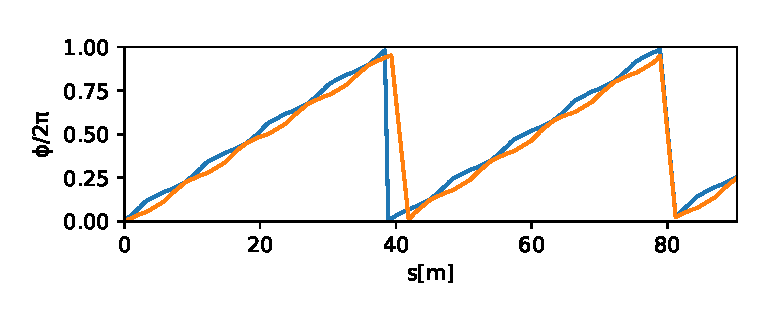
\includegraphics[width=1.0\textwidth]{phi.eps}
\end{figure}
Count the number of crossings, $\rm \nu_x$=2.25406 and $\rm \nu_y$=2.49926\\
\end{frame}
\begin{frame}
\frametitle{Analysis of TWISS output}
$\beta$ functions are also available.
\begin{figure}
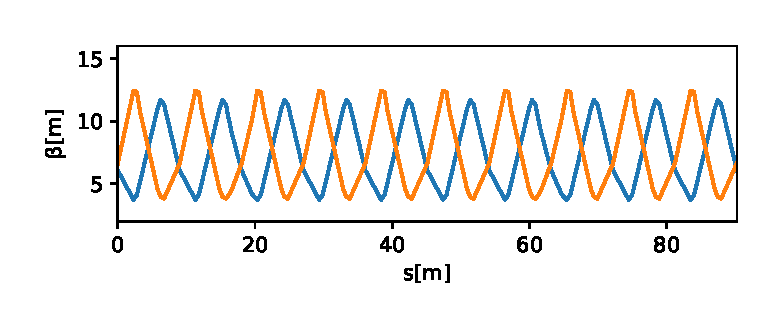
\includegraphics[width=1.0\textwidth]{beta.eps}
\end{figure}
For this lattice, $\rm \beta_{x,max}=11.68$, $\rm \beta_{x,max}=3.72$, $\rm \beta_{x,max}=12.44$, $\rm \beta_{x,max}=3.81$
\end{frame}

\section{3-Spin tracking}
\begin{frame}
\frametitle{3-Spin Tracking}
\begin{minipage}{1.0\textwidth}
\small
As calculated in "1-Exploring the Optics", the vertical betatron tunes  for the PSR is:
\vspace{-0.2em}
\begin{center}
$\rm\nu_y=2.2499$
\end{center}
\vspace{-0.2em}
Vertical intrinsic resonances occur when a particles betatron motion is in phase with the spin rotation or:
\vspace{-0.2em}
\begin{center}
$\rm G\gamma=NP+\nu_y$
\end{center}
\vspace{-0.2em}
where N=0, 1,... and P is the periodicity. A particles final vertical component after crossing a resonance can be described with the Froissart-Stora formula:
\begin{equation}
\frac{P_f}{P_i}=2\exp\bigg(-\frac{\pi|\epsilon_k|}{2\alpha}\bigg)-1
\end{equation}
where $\rm\epsilon_k$ is the resonance strength and $\rm \alpha=(G\Delta E)/(2\pi M_o)$ is the crossing speed.\\
So let's track a particle through the $G\gamma=0+\nu_y$ resonance.
\end{minipage}
\end{frame}
\begin{frame}
\frametitle{}
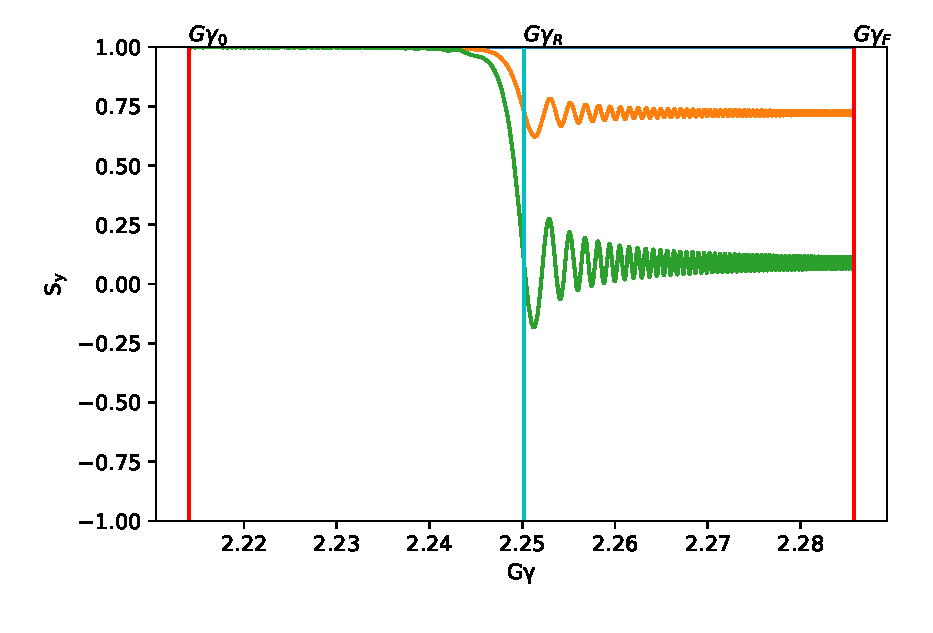
\includegraphics[width=1.0\linewidth]{PSR_FStora.eps}
\end{frame}
%\begin{frame}
%\frametitle{Notes about our new input file}
%\small
%Open up PSR.py file and not the change in syntax (this is using pyzgoubi).
%\begin{itemize}
%\item Lines up to \#70 are used to define lattice elements
%\item Lines \#71-94 are putting the elements together to create the lattice
%\item Lines \#102-119 are setting up the simulation and what will be in the zgoubi.dat file, and executing zgoubi
%\item Lines \#121-160 are used to calculate parameters for spin tracking
%\item Lines \#162 to end are used to setup spin tracking and execute zgoubi
%\end{itemize}
%Focusing quadrupole element is defined as:
%\tiny
%QUAD\_F=core.MULTIPOL("QUAD-F", R\_0=10.0, CS\_0=0.1122, S\_3=1, CS\_1=6.2671, CS\_2=-1.4982, CS\_3=3.5882, CS\_4=-2.1209, CS\_5=1.723, C\_0=0.1122, C\_1=6.2671, C\_2=-1.4982, C\_3=3.5882, C\_4=-2.1209, C\_5=1.723, B\_2=1.95*SCALING\_FACTOR\_0, E\_3=1, KPOS=1, XPAS=INT\_STEP, XL=50.0)\\
%\small
%and added to the lattice using:\\
%\tiny
%PSR\_Lattice.add(QUAD\_F)\\
%\small
%\end{frame}
\begin{frame}
\frametitle{What we need to calculate}

\begin{itemize}
\item Resonant $\rm G\gamma$ value, $\rm G\gamma_R$, and corresponding particle energy $\rm E_R$
\begin{itemize}
\item Used to determine where to center the simulation
\item The simulation is started $\rm N_{turns}$/2 turns away, where $\rm N_{turns}$ is the total number of turns for the tracking. 
\end{itemize}
\item Try $\rm N_{turns}=4000$
\item Change in energy per turn, $\Delta E$ calculated by RF parameters being used for tracking
\item Initial and final rigidities, $\rm B\rho_0$ and $\rm B\rho_F$
\begin{itemize}
\item Used to determine the scaling values at the start and end of the simulation.
\end{itemize}
\end{itemize}
%These parameters are calculated from lines \#126-167.\\
%Put a \# in front of line 126 and run PSR.py again to see the calculated values.
\end{frame}
\begin{frame}
\frametitle{Notes on your input file}
Magnet strengths have been scaled to a corresponding $B\rho$=1,000~kG cm.
\begin{itemize}
\item Scaling values $B\rho/1000$
\end{itemize}
SPNTRK sets the spin direction and tells zgoubi to track it.\\
CAVITE is for RF cavities and is in units of Volts.\\
REBELOTE tracks for $N_{turns}$-1.\\

%Run the input file in your terminal using:\\
%python PSR.py\\
%\vspace{1em}
%This portion of the file is used to get $\rm\nu_y$ for calculating $\rm G\gamma_R$\\
%\vspace{1em}
%The results $\rm\nu_y=2.24992584$ were printed to your shell, good.\\
%\vspace{1em}
%Open the file created named matrix.res and compare it to zgoubi.dat from the TWISS exercise.\\
%\vspace{1em}
%Parameters used are the same but the header of matrix.res was generated using python based off the parameters defined on the previous slide.

\end{frame}

\begin{frame}
\frametitle{Spin tracking}
We will track 3 particles with 3 different vertical betatron amplitudes:
\begin{itemize}
\item the reference particle has no vertical amplitude and should get $\rm P_f=P_i$
\item the 2 other particles have different amplitudes and should have different $\rm P_f$.
\end{itemize}
Tracking particles with RF voltage $\rm V_{cav}=15~kV$\\

%Put a \# in front of line 169 and run PSR.py again to see the calculated values.

\end{frame}

\begin{frame}
In your python shell run Fai\_plotter.py to analyze the results.
\hspace*{-2em}
\begin{minipage}{0.52\textwidth}
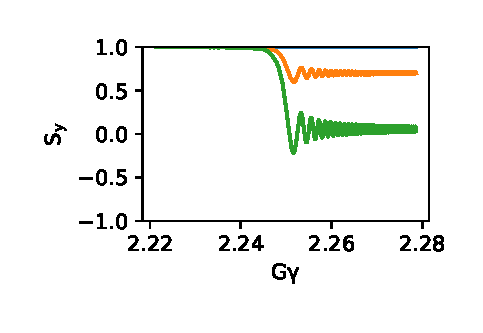
\includegraphics[scale=0.8]{PSR_SPNTRK.eps}
\end{minipage}
\begin{minipage}{0.48\textwidth}
\begin{tabular}{c|c|c}
Particle&$\rm P_f$&$\rm \epsilon_k\times 10^-3$\\
\hline
1&1.000&0.000\\
2&0.701&0.608\\
3&0.565&1.207\\
\end{tabular}
\end{minipage}
Try tracking particles with different amplitudes to see how $\rm P_f$ changes.\\
Track particles at different crossing speeds by adjusting $\rm V_{cav}$.
\end{frame}
\begin{thebibliography}{99}
\bibitem{AD1} Dragt, A. (1981). Exact Numerical Calculation of Chromaticity in Small Rings. Nuclear Science, IEEE Transactions on. 28. 2627 - 2629. 10.1109/TNS.1981.4331779. 
\bibitem{GPL} Lawrence, G. (1987). Performance of the Los Alamos Proton Storage Ring. Particle Accelerator Conference 1987.
\end{thebibliography}

\end{document}
